\chapter{Solution Design}
This chapter details and explains various aspects of the solution design. It begins with a explanation of the envisioned implementation of the solution in the clothing industry ecosystem. This is followed by a detailed account of the design process used to create the solution and lastly, an extensive overview of the experimental process used to test the solution.

\section{Implementation Design}

\subsection{Overview}
The solution aims to form part of larger practical implementation that will be applicable and provide relief in all three clothing channels mentioned in Section \ref{clothingIndustryContext}. However, in order to understand the needs the implementation must address, an analysis of pain points of consumers and producers in each channel must be performed. Shown in Table \ref{tab:conProdPainPoints} is a summary of such an analysis.

\begin{table}[htbp]
	\centering
	\caption{Pain points of consumers and producers in each of the three channels}
	\begin{tabularx}{\textwidth}{|Y|Y|Y|}
		\toprule
		& 
		\textit{\textbf{Consumers}} & 
		\textit{\textbf{Producers}} \\
		\midrule
		\textit{\textbf{Retail}} & 
		\begin{itemize}
			\item Visiting stores is time consuming
			\item Trying clothes on is tedious
			\item The correct size is often not available 
		\end{itemize} & 
		\begin{itemize}
			\item Dressing rooms waste valuable space
			\item Trying on clothes pose a security risk and require resources to control
			\item Significant costs are incurred during exchanges 
		\end{itemize} \\
		\midrule
		\textit{\textbf{Online}} & 
		\begin{itemize}
			\item Difficult to choose the correct size
			\item Not sure how the item will look on body
			\item Frustrating to exchange if item is incorrect
		\end{itemize} & 
		\begin{itemize}
			\item Exchanges severely impact their profitability
			\item Experience lower sale volume due as they cannot provide a complete customer experience
		\end{itemize}\\
		\midrule
		\textit{\textbf{Tailoring}} & 
		\begin{itemize}
			\item Only available for specialised clothing
			\item The process is time consuming
			\item There is always delay between getting measured and picking up clothing
		\end{itemize} & 
		\begin{itemize}
			\item Time required to complete measurements limits productivity
			\item Measurements can only take place in person with a trained tailor
		\end{itemize} \\
		\bottomrule
	\end{tabularx}%
	\label{tab:conProdPainPoints}%
\end{table}%


The aim of the overall implementation is to alleviate stresses on both consumers and suppliers that are inherent to the status quo.  In order to achieve this, the implementation will consist of the following key components: 

\begin{itemize}
	\item A compact, expedient and easy to use system that accurately measures the body parameters of a customer and provide clothing suggestions
	\item A platform that retains this customer information and creates a digital profile accessible to the customer and shareable between retailers  
	\item An intuitive interface that allows the customer to seamlessly get advise on clothing at his/her retailers of choice	
\end{itemize} 

These key components were developed into a more detailed end-to-end journey of the implementation. This is given in the following section.

\subsection{End-to-End Implementation Journey}
A diagram illustrating the high-level functioning of the entire implementation is seen in Figure \ref{fig:endToEndImplementation}.

\begin{figure}[ht]
	\centering
	{%
		\setlength{\fboxsep}{0pt}%
		\setlength{\fboxrule}{0.5pt}%
		\fbox{
			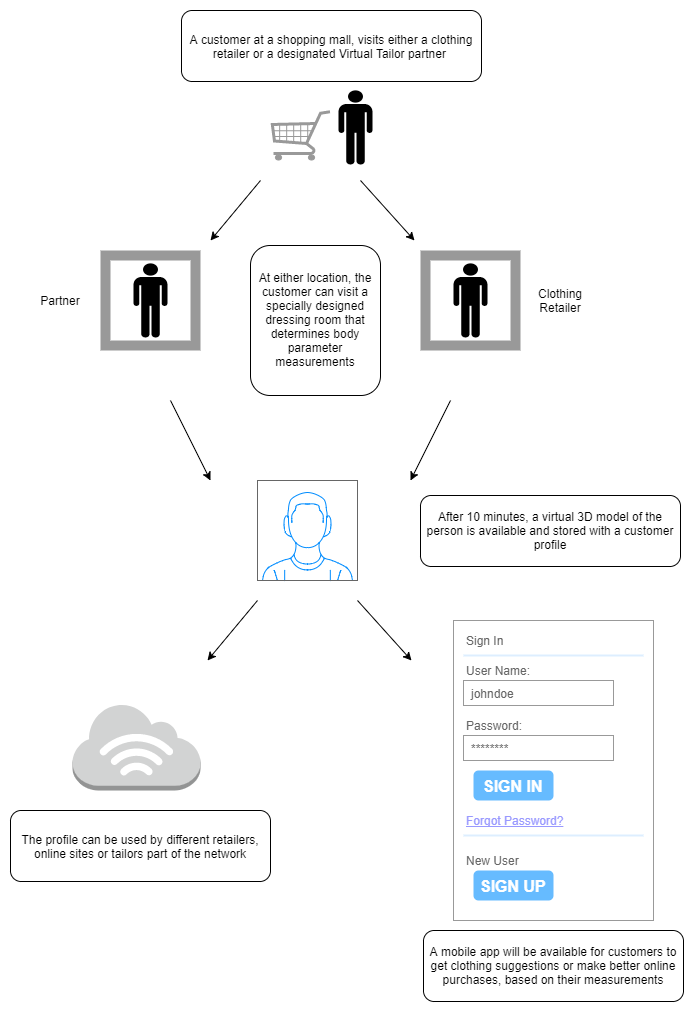
\includegraphics[width=0.7\textwidth]{End_to_End_Implementation.png}
	}}
	\caption{An illustration of the End-to-End journey of the envisioned implementation}
	\label{fig:endToEndImplementation}
\end{figure}

The implementation can be broken down into three major subsystems that are mentioned and explained in the following subsections:

\subsubsection{Measurement System}
This system's main purpose is to be able to determine the personalised body parameters of a customer and then generate a full 3D model of their body to provide useful information such as suggestions for clothing sizes. It will achieve this by using a Kinect, or another device with depth sensing capabilities. 

The vision is that the Kinect would be integrated into a specially designed room. The customer would need to step into this room and hold certain poses. The Kinect, together with a back-end processing unit, would then create a full 3D. The entire process from start to finish should be less than ten minutes. 

This is the most integral part of the implementation as it allows for the realisation of the other two subsystems mentioned below. The main focus of this project is creating a first attempt at this subsystem. As such, its design and functioning are covered in great detail in Section \hl{(Measurement Design)}. 

\subsubsection{Store Integration}
In order to facilitate the measuring process, a room, integrated with a Kinect, would need to be placed at a convenient location for customers. Two possibilities are explored here:

\paragraph{Traditional Retailers}
There is a significant incentive for these retailers to provide a space for this "virtual room". (Expanded upon in Section \hl{(Benefits)}) As such, given that this system aims to limit the need for physically trying on clothes, one of the spaces previously dedicated to a dressing room could be upgraded to this new virtual room. Minimal change to the infrastructure would be required and this also frees up more space as unused dressing rooms can be replaced. 

In this instance, consumers would be able to record their measurements when visiting the clothing store. The measurements would be recorded and they can continue their clothing shopping with a better understanding of sizes. Since the customer would already be shopping and the process only needs to occur once (Assuming no change to the customer's body), it seems likely that their would be buy-in into the system.

\paragraph{Partners}
If there is enough interest by various companies, a measurement booth can be built in a commonly used location (I.e. in a shopping mall). Any customer visiting this booth, would automatically have profiles at all the companies sharing the booth. This is the other alternative if a specific company does not want to dedicate their floor space for this solution, but rather outsource it. This would also be the most likely method in which an online store can partake to allow for digital profiles of their shoppers to be created.

\subsubsection{Cloud Management of Profile}
Once the measurements of a person are determined and a digital profile is created, that information can now be more easily transferred. Partnerships may be made between clothing companies, online companies and even perhaps tailors. They may agree to share this information for an agreed upon amount and allow the costumer to have clothing suggestions for all the stores they shop at. Alternatively, a single online platform may be created that stores all these profiles and if a clothing supplier partners up with it, it can then provide information to the customers regarding the supplier's specific line of clothing.

\subsubsection{title}

\subsubsection{title}
1) Online profile of people - Used for online shopping and retail shops\\
2) Take measurements at a retailer - Virtual Dressing room - A part of the shopping experience and will reduce hassle of trying on clothes\\
3) Amount wasted in trying on clothes or online returns?\\
4) Could be used for personalised tailoring
5) Example of UI - Explanation of how it works

\section{Component Level Design}


\section{Component Selection}
1) Choice of Kinect - Compare to other depth sensors\\
- Kinect v1 vs v2
- Winddows vs Xbox
2) Choice of Windows SDK\\

\section{Algorithm Design}
1) Windows examples used - Background Removal, Colour Stream and Skeleton Tracking - NB - Why BackgroundRemoval instead of own method
3D Points - No calibration

2) Run through of algorithm
- Background Removed frame
- Send image to separate class for processing
- Create array with background removed pixels
- Draw skeleton on image
- Create axes for measurement - Perpendicular or straight depending on particular measurement

\section{Experimental Design}
- Constraints - Men, distance from Kinect, height of Kinect, Number of views, 3D Modelling, control distance - box of 0.5m
- UI to run simulated dressing room
- Volunteer to pose as instructed by person controlling UI
- Take measurement of front
- Take left
- Take back
- Take right 
- At each point, take actual readings with uncertainty
- Note: Did not use correction in \cite{nonContact2017}
- For one volunteer, take 5 readings in relatively the same pose - Determine uncertainty 